\documentclass[border=3.14mm, tikz]{standalone}
\usetikzlibrary{3d,intersections}
\begin{document}

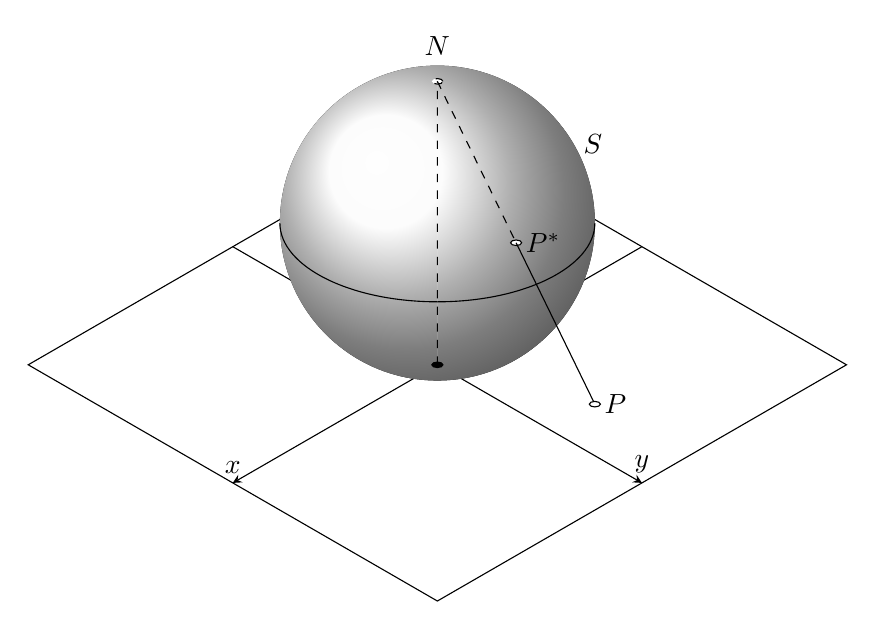
\begin{tikzpicture}[]
\pgfmathsetmacro{\angA}{60}
\pgfmathsetmacro{\angB}{30}
\pgfmathsetmacro{\lenA}{3}
\pgfmathsetmacro{\lenB}{3}
%
\draw(0,0)--(90-\angA:\lenA);
\draw[-stealth](0,0)--(-90-\angA:\lenA)node[above]{$x$};
\draw[-stealth](0,0)--(-\angB:\lenB)node[above]{$y$};
\draw(0,0)--(-\angB:-\lenB);
\draw(0,0)++(-\angB:\lenB)--++(90-\angA:\lenA)--++(-\angB:-2*\lenB)--++(90-\angA:-2*\lenA)--++(-\angB:2*\lenB)--++(90-\angA:\lenA);
%
\fill[ball color=white] (0,1.8) circle (2);
\shade[ball color=gray!10!white,opacity=0.25,name path global=circle] (0,1.8) circle(2);
\draw[fill=white,dashed](0,0)--(0,3.6)circle (2pt and 1pt)node[above,solid,yshift={(0.2cm)}]{$N$};
\draw[fill] (0,0)circle (2pt and 1pt);
\draw ([shift={(180:2cm and 1cm)}]0,1.8) arc (180:360:2cm and 1cm);
\path(0,3.6)--(2,-0.5)coordinate[pos=0.5](kA);
\draw[dashed](0,3.6)--(kA);
\draw[fill=white](kA)circle (2pt and 1pt)node[right]{$P^*$};
\draw[](kA)--(2,-0.5);
\draw[fill=white](2,-0.5)circle (2pt and 1pt)node[right]{$P$};
\draw(0,1.8)++(30:2)node[right]{$S$};
\end{tikzpicture}
\end{document}
